%% -*- coding:utf-8 -*-
\begin{figure}
\centering
\ifpdf
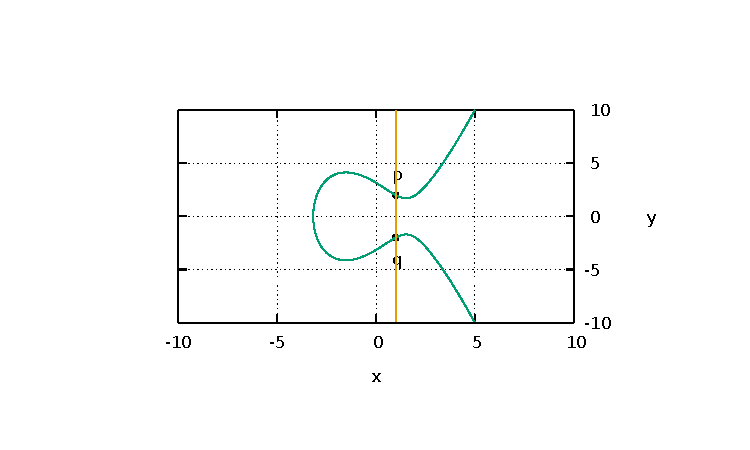
\includegraphics[angle=0,scale=1.5]
{./add/discretmath/picellipticsumeq.pdf}
\else
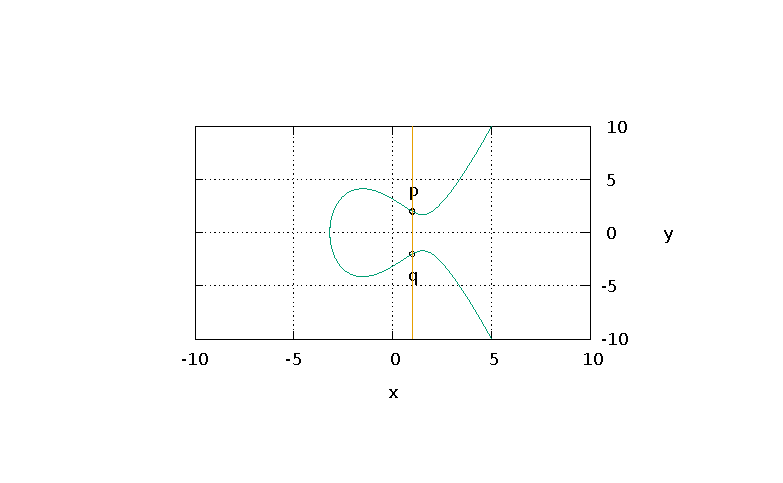
\includegraphics[angle=0,scale=1.5]
{./add/discretmath/picellipticsumeq.eps}
\fi
\caption{Эллиптическая кривая $y^2 = x^3 -7 x + 10$ над полем
  вещественных чисел $\mathbb{R}$. Сложение двух точек $p(1,2)$ и
  $q(1,-2)$. Прямая проходящая через эти точки не пересекает кривую.
  Результат сложения - нулевой элемент: $p + q = 0$, т.е. $q = -p$}
\label{fig:add:ellipticRsumEq}
\end{figure}
